O uso de conversores CC-CC é indicado quando deseja-se controlar um motor CC. A figura \ref{fig:C1-41-II} representa a estrutura básico desse conversor.

\begin{figure}[ht!]
\center
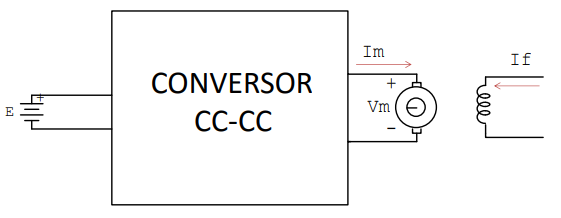
\includegraphics[scale= 0.88]{imagens/circuito1_41_II.png}
\caption{\label{fig:C1-41-II} Motor CC acionado por conversores CC-CC}
\caption*{Fonte: MARTINS, cap. 7, eslaide ARRUMAR.}
\end{figure}

Mesmo quando a fonte é de corrente alternada, o emprego dos conversores CC-CC pode ser muito interessante pois, em relação aos retificadores controlados, os conversores CC-CC operam com maior frequência, podendo assim obter condução contínua sem o emprego de filtros volumosos e a resposta torna-se mais rápida. 

